
\documentclass[utf8, 14pt]{beamer}


%%%%%%%%%%%%%%%%%%%%%%%%%%% FANCYHDR %%%%%%%%%%%%%%%%%%%%%%%%%%%%%%

\lhead{I3 - S9}
%\lhead{
\includegraphics[scale=0.4]{images/eseo.jpg}} % Logo Eseo
\chead{Synthèse}
\rhead{\today}
\lfoot{}
\cfoot{\thepage /\pageref{LastPage}}
\rfoot{}%\LaTeX

%\renewcommand{\headrulewidth}{0pt} % Taille des traits entete et pied de page
%\renewcommand{\footrulewidth}{0.4pt}

				%%%%%%%%%%%%%%%%%%%%%%%%%%%%%%%%%

\title{\Huge{\textbf{Design Patterns - Incrément 6}}}
\author{
	\Large{Axel \textsc{Gendillard}}\\
	\Large{Audoin \textsc{De Chantérac}}
}
\date{}

%%%%%%%%%%%%%%%%%%%%%%%%%%%%%%%%%%%%%%%%%%%%%%%%%%%%%%%%%%%%%%%%%%%

\definecolor{javared}{rgb}{0.6,0,0} % for strings
\definecolor{javagreen}{rgb}{0.25,0.5,0.35} % comments
\definecolor{javapurple}{rgb}{0.5,0,0.35} % keywords
\definecolor{javadocblue}{rgb}{0.25,0.35,0.75} % javadoc
\definecolor{javagrey}{rgb}{0.95,0.95,0.95} % background
 
\lstset{language=Java,
basicstyle=\ttfamily,
keywordstyle=\color{javapurple}\bfseries,
stringstyle=\color{javared},
commentstyle=\color{javagreen},
morecomment=[s][\color{javadocblue}]{/**}{*/},
backgroundcolor = \color{javagrey},
% numbers=none,
% numberstyle=\tiny\color{black},
% stepnumber=2,
% numbersep=10pt,
tabsize=4,
showspaces=false,
showstringspaces=false}


%%%%%%%%%%%%%%%%%%%%%%%% NEWCOMMAND %%%%%%%%%%%%%%%%%%%%%%%%%%%%%%

%\newcommand{}{}
%\renewcommand{}{}



%%%%%%%%%%%%%%%%%%%%%%%%%%%%%%%%%%%%%%%%%%%%%%%%%%%%%%%%%%%%%%%%%%%


%%%%%%%%%%%ù%%%%%%%%%%%% NEWENVIRONEMENT %%%%%%%%%%%%%%%%%%%%%%%%%%

%\newenvironment{•}{•}{•}
%\renewenvironment{•}{•}{•}

%% Configuration de l'environnement gbar %%

%\newenvironment{gbar}[1]{\def \FrameCommand{{\color{#1} \vrule width 4pt }\colorbox{lightgray!70}}\MakeFramed{\advance \hsize - \width \FrameRestore}}{\endMakeFramed}


%%%%%%%%%%%%%%%%%%%%%%%%%%%%%%%%%%%%%%%%%%%%%%%%%%%%%%%%%%%%%%%%%%%


%%%%%%%%%%%%%%%%%%%%% POINTILLÉ SOMMAIRE %%%%%%%%%%%%%%%%%%%%%%%%%%


					% Sans chapitre %

%\makeatletter
%\renewcommand\l@section[2]{%
%\ifnum \c@tocdepth >\z@
%\addpenalty\@secpenalty
%\addvspace{1.0em \@plus\p@}%
%\setlength\@tempdima{1.5em}%
%\begingroup
%\parindent \z@ \rightskip \@pnumwidth
%\parfillskip -\@pnumwidth
%\leavevmode {\bfseries
%\advance\leftskip\@tempdima
%\hskip -\leftskip
%#1}\nobreak\ 
%\leaders\hbox{$\m@th\mkern \@dotsep mu\hbox{.}\mkern \@dotsep mu$}
%\hfil \nobreak\hb@xt@\@pnumwidth{\hss #2}\par
%\endgroup
%\fi}
%\makeatother


					% Avec chapitre %

%\makeatletter
%\renewcommand*\l@chapter[2]{%
%\ifnum \c@tocdepth >\m@ne
%\addpenalty{-\@highpenalty}%
%\vskip 0.5em \@plus\p@
%\setlength\@tempdima{1.5em}%
%\begingroup
%\parindent \z@ \rightskip \@pnumwidth
%\parfillskip -\@pnumwidth
%\leavevmode \bfseries
%\advance\leftskip\@tempdima
%\hskip -\leftskip
%#1\nobreak\ 
%\leaders\hbox{$\m@th
%\mkern \@dotsep mu\hbox{{\scriptsize .}}\mkern \@dotsep
%mu$}\hfil\nobreak\hb@xt@\@pnumwidth{\hss #2}\par
%\penalty\@highpenalty
%\endgroup
%\fi}
%\makeatother

%%%%%%%%%%%%%%%%%%%%%%%%%%%%%%%%%%%%%%%%%%%%%%%%%%%%%%%%%%%%%%%%%%%

%----------------------------------------------------------------------------------------
%	TITLE PAGE
%----------------------------------------------------------------------------------------

\title[Design Patterns]{Design Patterns}
\subtitle{OS Virtuel}

\author[Axel G. | Audoin De C.]{Axel \textsc{Gendillard} \and Audoin \textsc{De Chantérac}}
\institute[]
{
	Étudiant ingénieur\\ 
	Groupe ESEO \\
	%\medskip
	%\textit{axel.gendillard@reseau.eseo.fr}
}

\date{\today} 

%\logo{\includegraphics[scale=0.3]{logo}}

\titlegraphic{%
%\includegraphics[scale=0.55]{logo} \hspace{1cm}~%
%
\includegraphics[scale=0.6]{eseo}
}


\begin{document}

\begin{frame}
\titlepage
\end{frame}

\begin{frame}{Sommaire}
\tableofcontents
\end{frame} 

%----------------------------------------------------------------------------------------
%	PRESENTATION SLIDES
%----------------------------------------------------------------------------------------

\section{Incrément 1 : Singleton}
	
	\begin{frame}{Incrément 1 : Singleton}
		\begin{block}{Objectifs}
		\begin{itemize}
		\item Créer un nouvel utilisateur à chaque validation;
		\item Avoir un utilisateur unique par login;
		\item Créer plusieurs terminaux par utilisateur;
		\item Interdir la création d'utilisateur hors de la fenêtre.
		\end{itemize}
		\end{block}
		
		\begin{exampleblock}{Patron Singleton}
		\begin{itemize}
		\item Garantir l'unicité de l'instance d'une classe;
		\item Accéder globalement à l'instance.
		\end{itemize}
		\end{exampleblock}					
	\end{frame}

	\begin{frame}{Incrément 1 : Singleton - UML}
		\begin{figure}[!h]
		\centering
		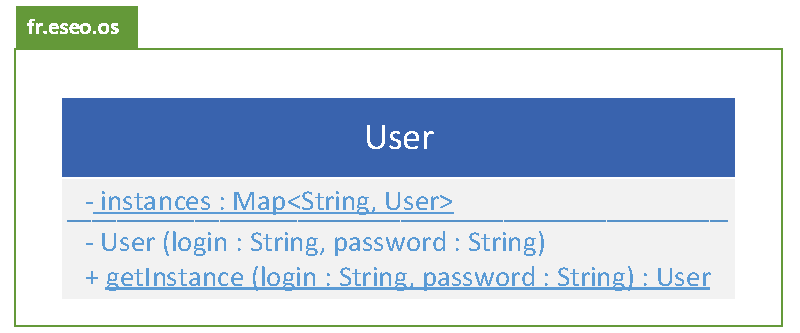
\includegraphics[width=\textwidth]{../uml/uml-singleton}
		\end{figure}		
	\end{frame}


\section{Incrément 2 : Observer}
	
	\begin{frame}{Incrément 2 : Observer}
		\begin{block}{Objectifs}
		\begin{itemize}
		\item Synchroniser les historiques des terminaux;
		\item Mettre à jour tous les terminaux lors de l'entrée d'une commande.
		\end{itemize}
		\end{block}
		
		\begin{exampleblock}{Patron Observer}
		\begin{itemize}
		\item Permet de mettre à jour les objets observés en fonction de l'objet observateur.
		\end{itemize}
		\end{exampleblock}					
	\end{frame}

	\begin{frame}{Incrément 2 : Observer - UML}
		\begin{figure}[!h]
		\centering
		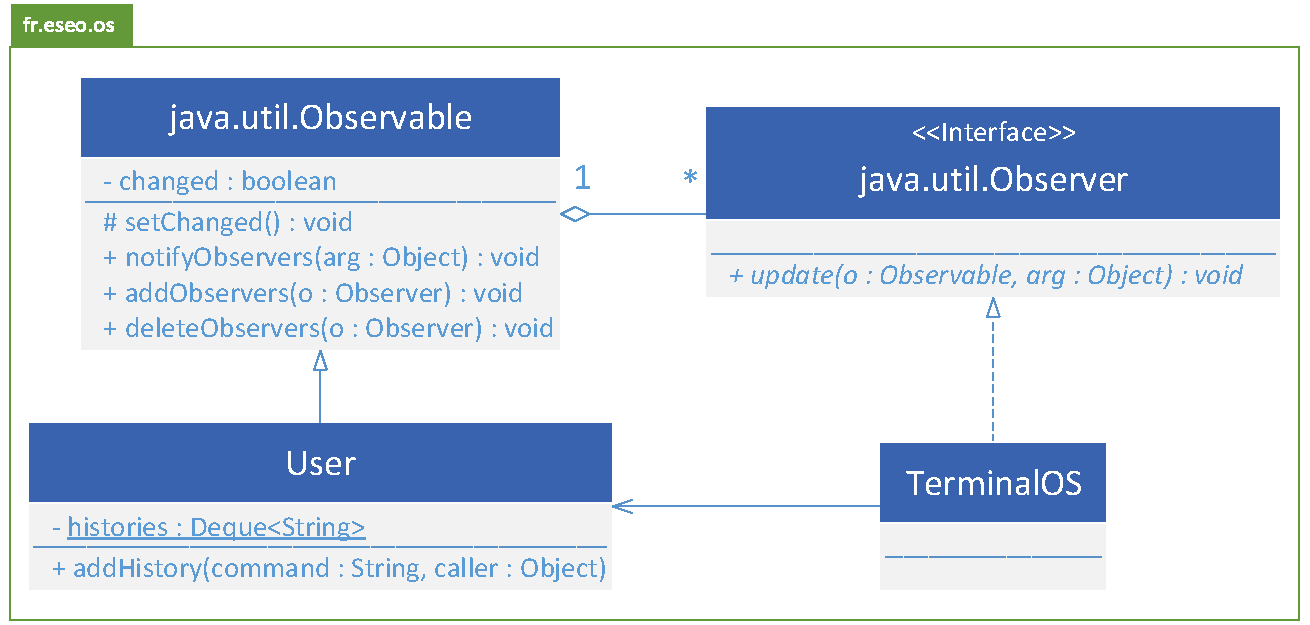
\includegraphics[width=\textwidth]{../uml/uml-observer}
		\end{figure}		
	\end{frame}



\section{Incrément 3 : Visiteur}
	
	\begin{frame}{Incrément 3 : Visiteur}
		\begin{block}{Objectifs}
		\begin{itemize}
		\item Interpréter des commandes du terminal (ls et cat) pour chaque type de noeud;
		\item Utiliser le patron Visitor.
		\end{itemize}
		\end{block}
		
		\begin{exampleblock}{Patron Visiteur}
		\begin{itemize}
		\item Sépare l'algorithme de la structure de données;
		\item Chaque élément implémente une méthode d'acceptation de visiteur;
		\item Chaque visiteur implémente une méthode \emph{visit()} pour chaque élément (file, folder et link).
		\end{itemize}
		\end{exampleblock}					
	\end{frame}

	\begin{frame}{Incrément 3 : Visiteur - UML}
		\begin{figure}[!h]
		\centering
		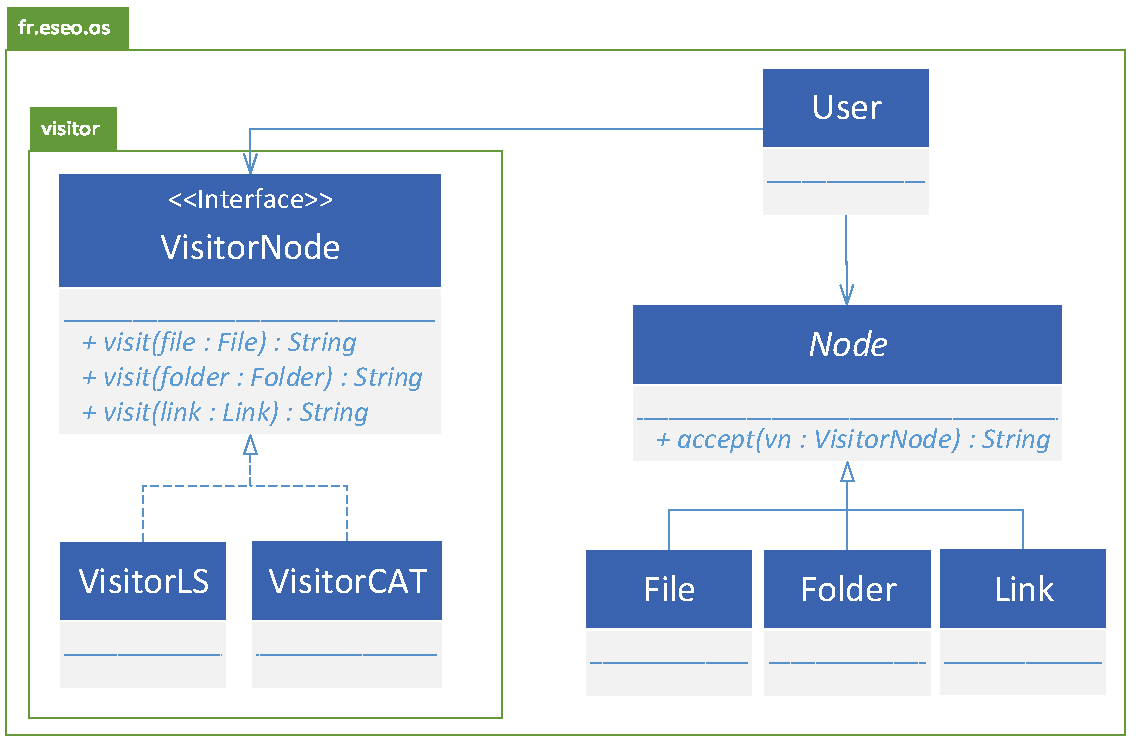
\includegraphics[width=\textwidth]{../uml/uml-visitor}
		\end{figure}		
	\end{frame}


\section{Incrément 4 : Commande}
	
	\begin{frame}{Incrément 4 : Commande}
		\begin{block}{Objectifs}
		\begin{itemize}
		\item Réutiliser les traitements interprétés par le terminal;
		\item Exprimer de manière unique le traitement des commandes ls et cat.
		\end{itemize}
		\end{block}
		
		\begin{exampleblock}{Patron Commande}
		\begin{itemize}
		\item Isole une requête;
		\item Ces requêtes peuvent provenir de plusieurs émetteurs (\emph{TerminalOS} et \emph{ExplorerOS});
		\item Ces émetteurs doivent produire la même requête;
		\item Ces requêtes doivent pouvoir être annulées.
		\end{itemize}
		\end{exampleblock}					
	\end{frame}

	\begin{frame}{Incrément 4 : Commande - UML}
		\begin{figure}[!h]
		\centering
		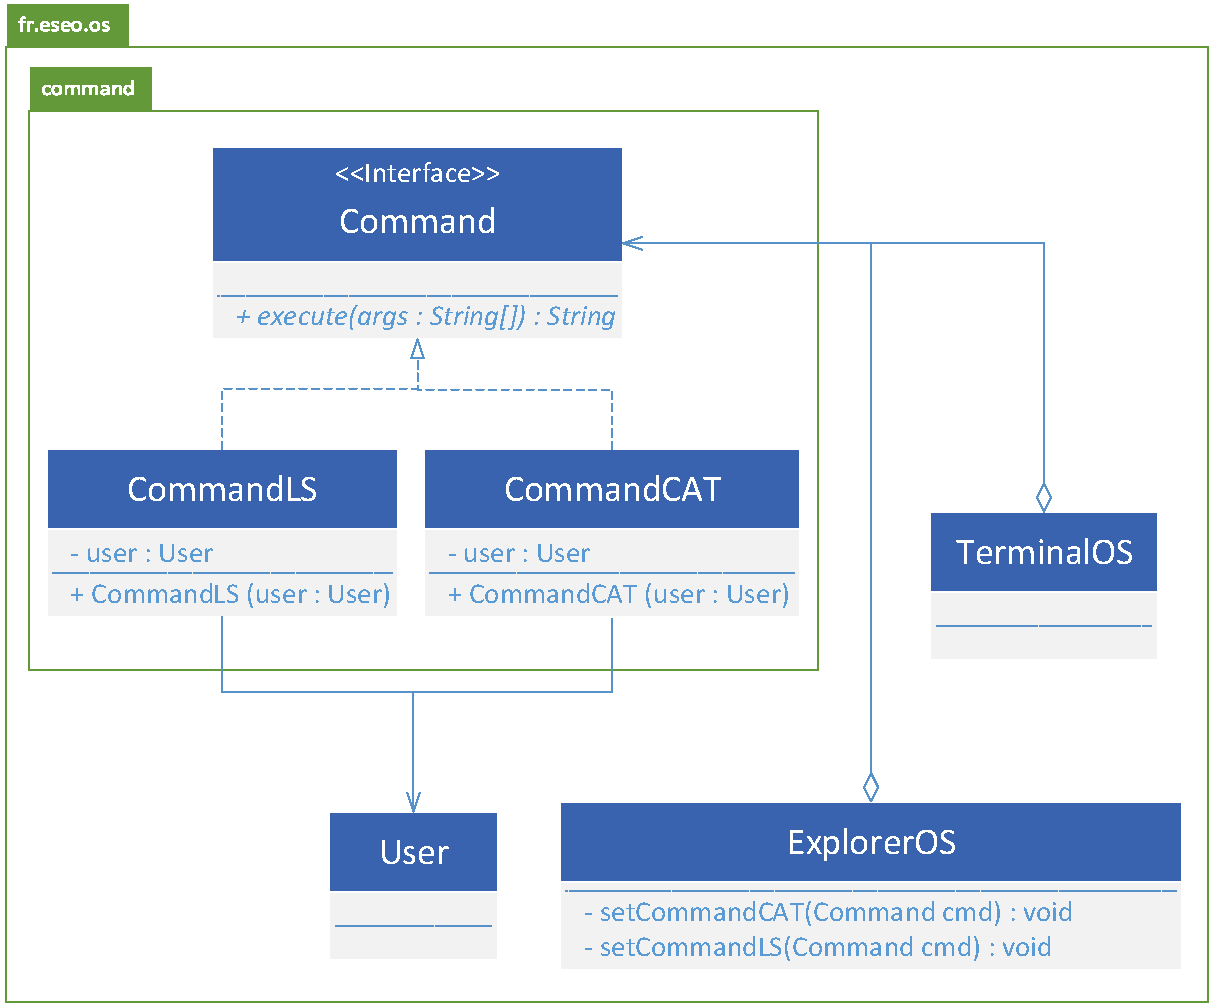
\includegraphics[width=0.78\textwidth]{../uml/uml-command}
		\end{figure}		
	\end{frame}

\section{Incrément 5 : Commande ++}
	
	\begin{frame}{Incrément 5 : Commande ++}
		\begin{block}{Objectifs}
		\begin{itemize}
		\item RM : Supprimer un dossier, un fichier ou un lien;
		\item MKDIR : Créer un dossier;
		\item TOUCH : Créer un fichier;
		\item LN : Créer un lien.
		\end{itemize}
		\end{block}
		
		\begin{exampleblock}{Patron Commande}
		\begin{itemize}
		\item Isole une requête;
		\item Ces requêtes peuvent provenir de plusieurs émetteurs (\emph{TerminalOS} et \emph{ExplorerOS}) ayant le même focntionnement;
		\item Ces requêtes doivent pouvoir être annulées.
		\end{itemize}
		\end{exampleblock}					
	\end{frame}

	\begin{frame}{Incrément 5 : Commande - UML}
		\begin{figure}[!h]
		\centering
		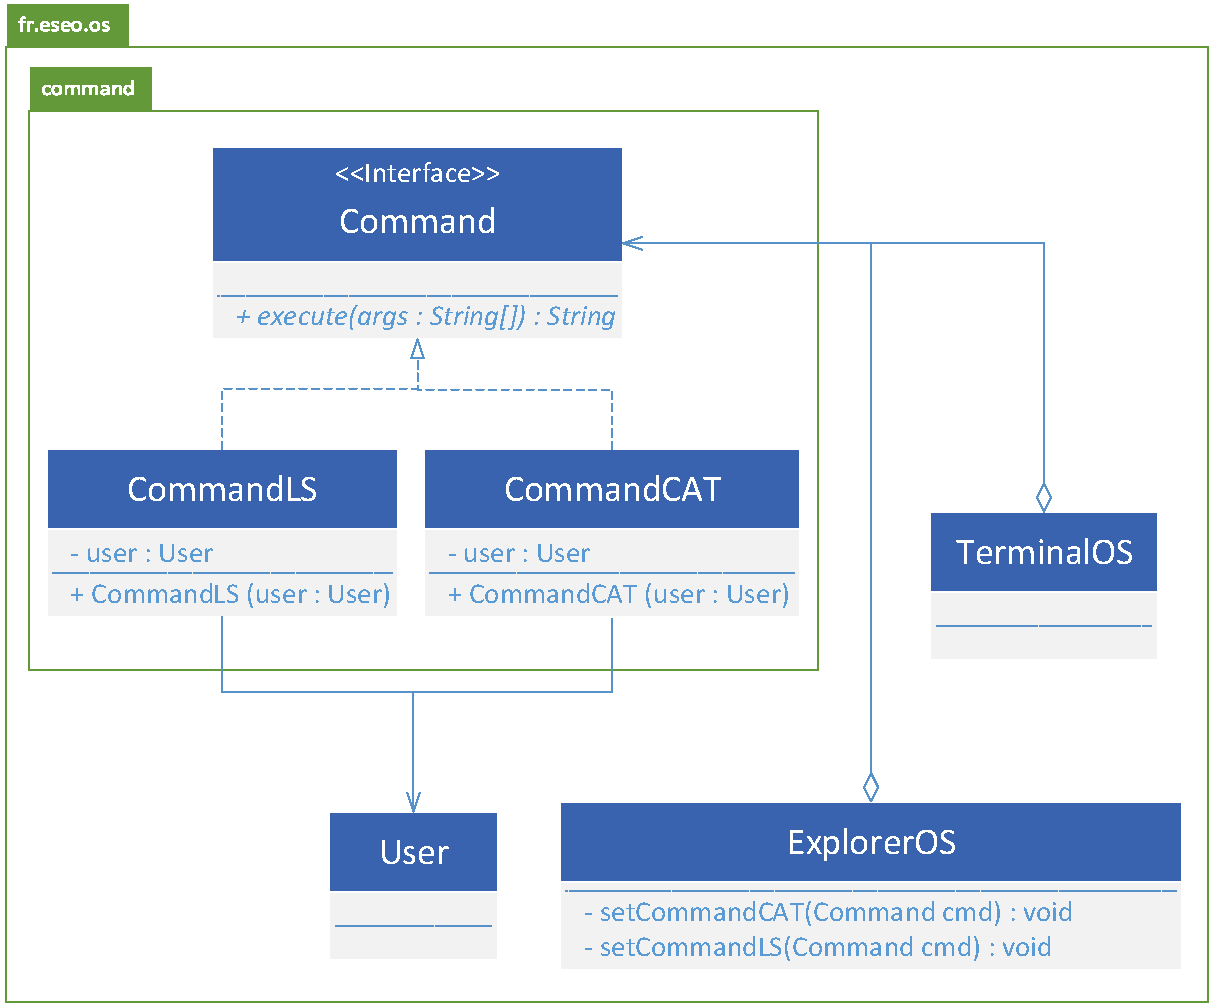
\includegraphics[width=0.78\textwidth]{../uml/uml-command}
		\end{figure}		
	\end{frame}

\section{Incrément 6 : Proxy}
	
	\begin{frame}{Incrément 6 : Proxy}
		\begin{block}{Objectifs}
		\begin{itemize}
		\item Lecture seule : Pas de modification des données des utilisateurs ls et cat sont autorisées;
		\item Lecture/écriture : Les commandes mkdir, touch, ln et rm sont autorisées.
		\end{itemize}
		\end{block}
		
		\begin{exampleblock}{Patron Proxy}
		\begin{itemize}
		\item Rôle d'aiguilleur en fonction des droits de l'utilisateur;
		\item Couche d'abstraction entre le client et la commande.
		\end{itemize}
		\end{exampleblock}					
	\end{frame}

	\begin{frame}{Incrément 6 : Proxy - UML}
		\begin{figure}[!h]
		\centering
		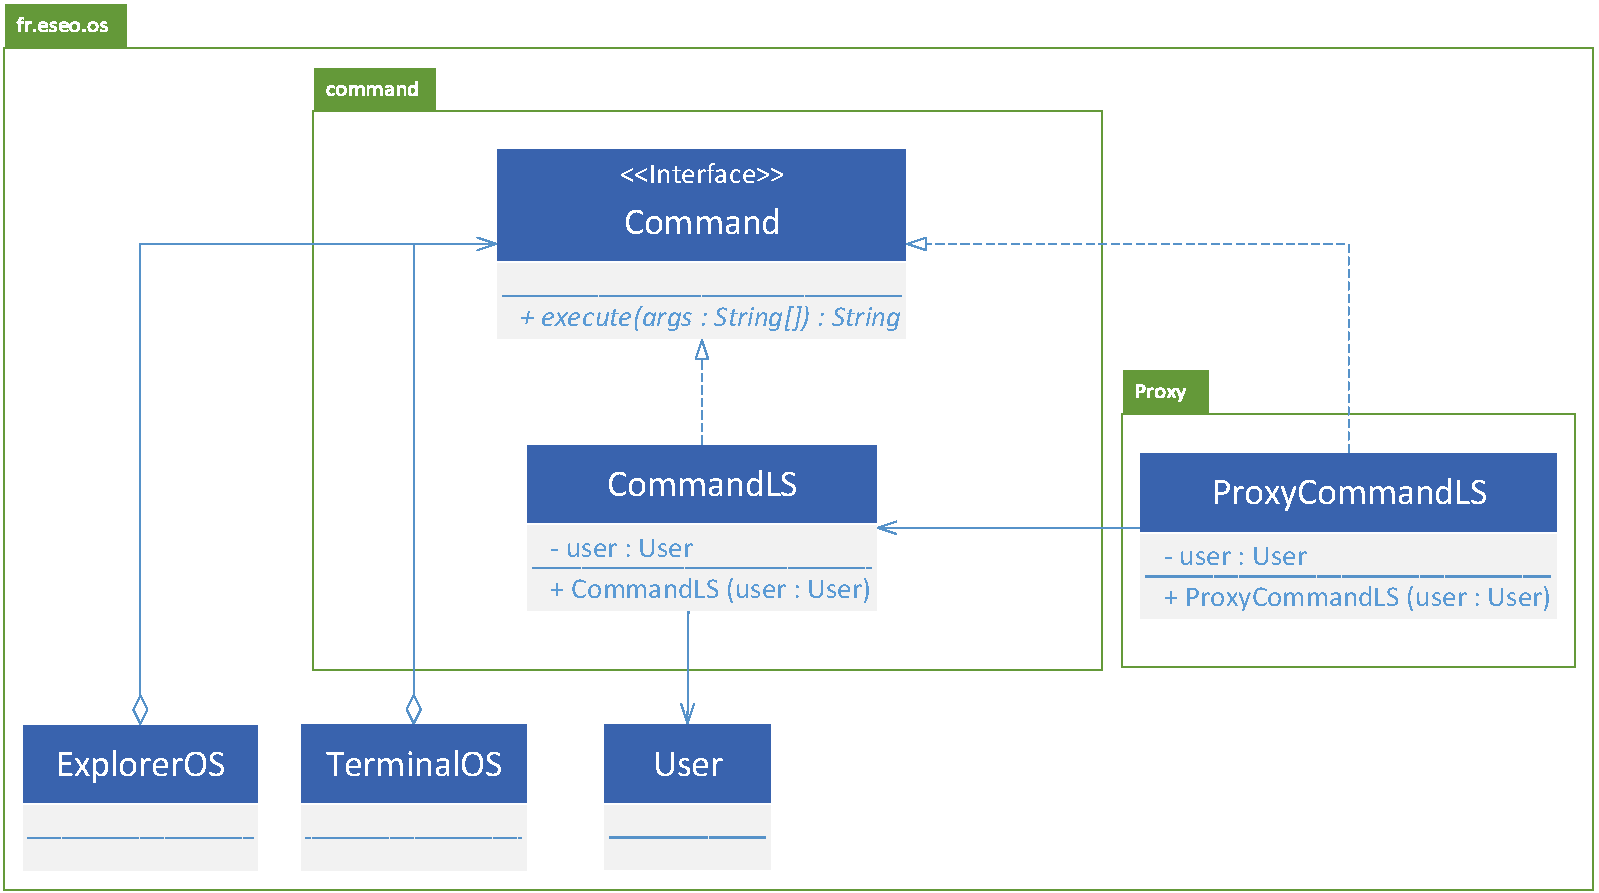
\includegraphics[width=\textwidth]{../uml/uml-proxy}
		\end{figure}		
	\end{frame}

	\section{Bonus : Gestion de l'historique au clavier}
	
	\begin{frame}{Bonus : Gestion de l'historique au clavier}
		\begin{block}{Objectifs}
		\begin{itemize}
		\item Implémenter un gestionnaire d’historique au clavier (flèche du haut et du bas)
		\item Utiliser la classe \emph{java.awt.event.KeyAdapter}
		\end{itemize}
		\end{block}
		
		\begin{exampleblock}{Implémentation}
		\begin{itemize}
		\item Création classe \emph{KeyBoardListener} qui hérite de \emph{KeyAdapter}
		\item Création d'un \emph{listener} sur les événement du clavier
		\item La méthode \emph{handleCommand()} est appelée via la touche \emph{Enter}.
		\end{itemize}
		\end{exampleblock}					
	\end{frame}

	\begin{frame}{Bonus : UML}
		\begin{figure}[!h]
		\centering
		\includegraphics[width=0.95\textwidth]{../uml/uml-keyboard}
		\end{figure}		
	\end{frame}

	\begin{frame}{Bonus : Un peu de code pour finir}
		\begin{figure}[!h]
		\centering
		\includegraphics[width=\textwidth]{../uml/code}
		\end{figure}		
	\end{frame}


\end{document} 
